\chapter{Evaluation and results}

    \section{Benchmarking}

        % the metdata benchmark is an IO benchmark. Argue this.

        Benchmarking a file system involves many aspects and different authors
        have done it in varying ways over the years.  \citeauthor{FFS} measures
        raw throughput of data, \citeauthor{LFS} recorgnise both small reads
        and writes as well as long sustained accesses.
        \citeauthor{soft_updates} on the other hands looks at speed of metadata
        access and modificaiton while \citeauthor{ext4_space_maps} uses a small
        file benchmark that simulates and email server. Finally, Google use a
        hybrid approach where they try a large variety of real world
        representative data with a large distribution of sizes. In the mean
        time popular consumer review sources add random accesses to the mix
        \cite{servethehome_review}, IO operations per second (IOPS)
        \cite{tomshardware_review} and many other ways of looking at
        performance of drives. These last methods are a bit different in that
        they measure drive performance without usually varying the filesystem
        but they are still representative as they aim to find bottlenecks and
        measure the performance of likely usecases.

        Despite the variety of test methodologies the important metrics for
        filesystems and SSDs become apparent: the raw read and write throughput
        and the number of individual IO requests they can fulfill. This is
        measured in the extremes and in various combinations of the two to
        represent different use cases like metadata access, office work or
        fileserver workloads.

        To measure these a utility written by the author of the new Linux
        system call interface io\_uring, \citeauthor{IO_uring}, is used - fio
        \cite{fio}. Using fio a test is devised to test the critical points
        that the above test for: random IO, sequential IO and metadata
        modificaiton. This is implemented as 8 'jobs' - individual tasks that
        fio completes. A Read, a write and a combined test for both small (4K
        size) and large (1M size) files, for a total of 6.  Then a sequential
        read and write test of 1GB of data and finally creating and removing
        100 files in a loop. Each of these tests is perfomerd in sequence for
        20 seconds each.

        All tests are perfomerd using the same hardware and sofware setup: a
        loopback device is set up using a regular file on the filesystem as a
        backing store. The drive is a "SAMSUNG MZVLB1T0HBLR-000L7" high speed
        NVMe drive tested on an AMD Ryzen 7 PRO 4750U CPU. The test was ran 3
        times and average values were taken. As controls two more filesystems
        were tested: ext4 and ntfs (with the ntfs-3g driver). They represent
        two of the most modern filesystems used today and are the main
        competitors to the this project (as described in section \ref{???; idk
        if i say it there}. All tests were performed by completely wiping each
        drive before commencing for consistency.

    \section{Test results}

        The results of the benchmark above are in figure \ref{fig_benchmark}.
        Combined read and write tests have the read and write components added
        toghether in the summary. The raw data for the graph can be found in
        appendinx \ref{app_benchmark}.

        % \begin{wrapfigure}{L}{0.2\textwidth}
        % \end{wrapfigure}
        \begin{figure}[h!]
            \caption{Benchmark results}
            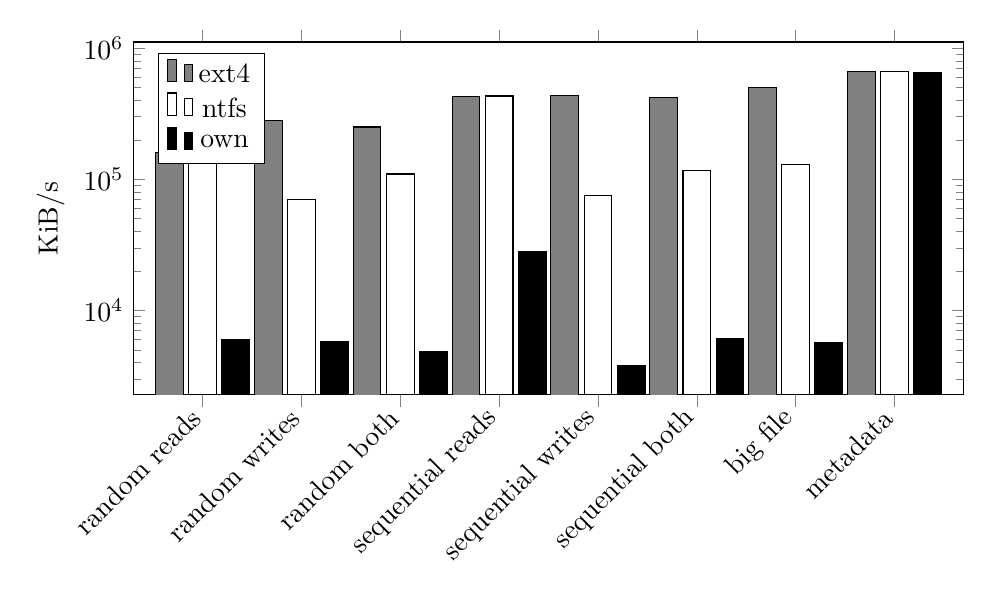
\begin{tikzpicture}
\begin{axis} [
    ybar, ymode = log,
    ylabel = {KiB/s},
    width=\textwidth, height = 0.5\textwidth,
    % scale only axis,
    symbolic x coords = {
        random reads, random writes, random both,
        sequential reads, sequential writes, sequential both,
        big file, metadata
    },
    x tick label style = {rotate = 45, anchor = east},
    legend pos = {north west}
]

    % ext
    \addplot[
        fill=gray,
    ] coordinates {
        (random reads, 159403) (random writes, 280917) (random both, 250539)
        (sequential reads, 430421) (sequential writes, 432469) (sequential both, 417792)
        (big file, 497323) (metadata, 663893)
    };

    % ntfs
    \addplot[
    ] coordinates {
        (random reads, 162133) (random writes, 70519) (random both, 109670)
        (sequential reads, 431445) (sequential writes, 74684) (sequential both, 116395)
        (big file, 128956) (metadata, 664576)
    };

    % own
    \addplot[
        fill=black,
    ] coordinates {
        (random reads, 5963) (random writes, 5812) (random both, 4820)
        (sequential reads, 28331) (sequential writes, 3799) (sequential both, 6104)
        (big file, 5693) (metadata, 651947)
    };

    \legend{ext4, ntfs, own};

\end{axis}
\end{tikzpicture}

            \label{fig_benchmark}
        \end{figure}

        The ext4 and ntfs controls appear to behave as expected. Their
        performance is comparable although ntfs performs worse across the board
        as it is natively implemented on Windows and the Linux driver has
        historically been lagging behind. Regardless, the ext4 results are a
        best case maximum whereas the ntfs ones are a more realistic
        representation of an in-kernel but imperfect filesystem.

        The proposed filesystem's performs an order of magnitude lower across
        the board. As discussed in the design stage (\ref{sec_design})
        performance was expected to be worse. Random reads and writes are of
        comparable speed. This is not surprising, as the code paths they take
        are similar. Each access needs to have its destination resolved and
        then data written in the same way. Interestingly, however, sequential
        reads are about an order of magnitude higher than the overall
        perfomance of the filesystems and the corresponding sequential writes.
        This cannot be attributed to drive assymetry, as the difference tends
        to be linear in SSDs \cite{servethehome_review}. Ext4 handles both
        workloads identially, indicating that is not the case. The ntfs-3g
        driver is a reverse engineering effort of the proprietary ntfs
        filesystem and has been notorious for having a problematic
        implementation. To confirm this, we perform profiling analysys in
        \ref{sec_perf}.

    \section{Failure simulation}

    \section{Reliability}

        probabilistic, not a guarantee like ZFS. ZFS is a "blockchain" I just
        minimise the likelyhood by many orders of magnitude

    \section{Comparison to existing alternatives}
